\section{The LIGO Detectors and GW150914} \label{sec:2}
\subsection{Interferometric Detection of Gravitational Waves}

Gravitational waves are transverse perturbations of spacetime curvature that propagate at the speed of light. In the transverse–traceless (TT) gauge, a passing gravitational wave induces differential strain in orthogonal spatial directions. The observable quantity measured by ground-based detectors is the dimensionless strain
\begin{equation}
	h(t) = \frac{\Delta L(t)}{L},
\end{equation}
where $L$ is the interferometer arm length and $\Delta L(t)$ is the differential change in arm lengths induced by the gravitational wave\cite{Abbott2016Discovery}.

The Laser Interferometer Gravitational-Wave Observatory (LIGO) detectors are kilometer-scale Michelson interferometers with Fabry–Pérot arm cavities designed to measure strains on the order of $10^{-21}$. Each detector consists of two perpendicular 4 km arms. A passing gravitational wave stretches one arm while compressing the other, producing a measurable phase shift in the recombined laser light
\cite{Abbott2016Discovery}.

The strain sensitivity of LIGO is frequency-dependent and the most sensitive band is 100 to 300 Hz. At low frequencies, seismic noise dominates, while at high frequencies shot noise and quantum noise become significant. For binary black hole mergers such as GW150914, the majority of detectable signal power lies between approximately 30 Hz and 300 Hz, which motivates the frequency band used later in this analysis
\cite{Aasi2015AdvancedLIGO,Abbott2016Discovery}.
\subsection{The Hanford and Livingston Observatories}

LIGO operates two geographically separated detectors in the United States: the LIGO Hanford Observatory (H1) in Washington and the LIGO Livingston Observatory (L1) in Louisiana. The two observatories are separated by approximately 3000 km. This separation is essential for distinguishing true astrophysical signals from local instrumental or environmental disturbances \cite{Abbott2016Properties}.

A gravitational wave arriving from an astrophysical source will be observed in both detectors with a relative time delay determined by the source sky location, the orientation of each interferometer, and the propagation speed of gravitational waves (consistent with the speed of light)\cite{Abbott2016Properties}. Because the light travel time between the two sites is about 10 milliseconds, the maximum possible arrival time difference between H1 and L1 is approximately $\pm 10$ ms. Therefore, measuring an inter-detector delay within this range provides strong evidence for an astrophysical origin.

The detectors are not perfectly co-aligned; their antenna response patterns differ slightly due to their orientations. Consequently, the measured strain amplitudes in H1 and L1 are not identical, although the waveform morphology remains consistent\cite{Abbott2016Discovery}.

\begin{figure}[h]
	\centering
	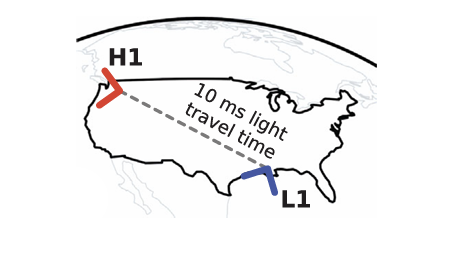
\includegraphics[width=0.4\textwidth]{figure/ligo_map}
	\caption{Geographic locations of the Hanford and Livingston observatories\cite{Abbott2016Discovery}.}
\end{figure}


\subsection{The Event GW150914}

The gravitational-wave event GW150914 was the first direct detection of gravitational waves, observed on 14 September 2015 at GPS time 1126259462.4. The signal originated from the merger of two stellar-mass black holes with component masses of approximately $36\,M_{\odot}$ and $29\,M_{\odot}$. The event marked the first direct observation of a binary black hole system and provided strong confirmation of general relativity in the strong-field regime\cite{Abbott2016Discovery, Abbott2016Properties}.

In the detector band, GW150914 appears as a short-duration chirp lasting roughly 0.2 seconds, with frequency sweeping from approximately 35 Hz to about 250 Hz. This characteristic frequency evolution makes the event well-suited for both time--frequency analysis and matched filtering techniques.

\subsection{Physical Expectations for the Present Analysis}

Before performing the data analysis, several physical expectations guide the interpretation:

\begin{enumerate}
	\item \textbf{Coincident detection:} The signal must appear in both H1 and L1.
	\item \textbf{Finite time delay:} The inter-detector delay should be less than 10 ms.
	\item \textbf{Chirp signature:} The signal should exhibit a monotonic increase in frequency over time.
	\item \textbf{Template consistency:} Matched filtering with a physically motivated waveform should yield a high signal-to-noise ratio (SNR).
	\item \textbf{Statistical consistency:} A chi-square test should indicate that the signal’s frequency content matches the theoretical template.
\end{enumerate}

The following sections evaluate these expectations using publicly available LIGO strain data.
